% Model Comparison Forest Plot (Brier Score + ATS%)
% Complements: tab:benchmark-comparison
% Shows our models vs published benchmarks with visual comparison

\begin{figure}[htbp]
\centering
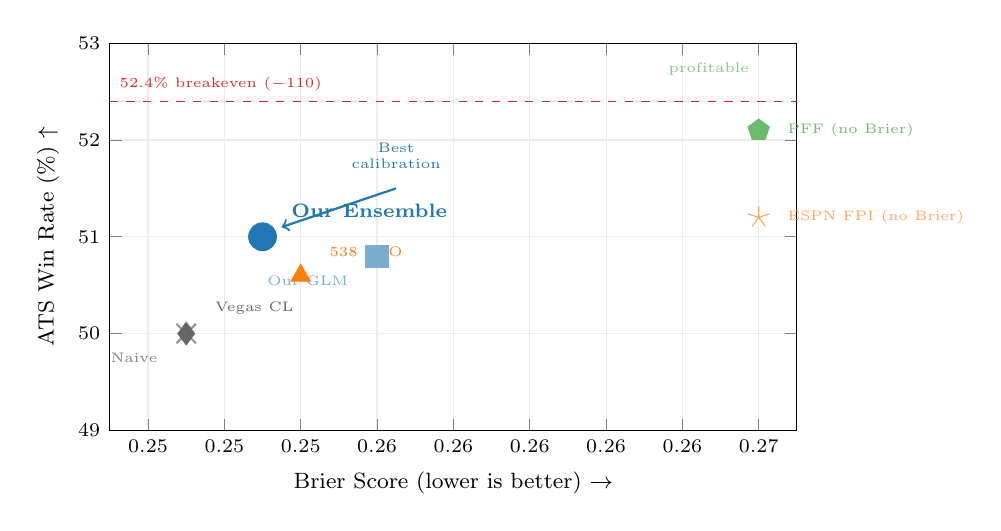
\begin{tikzpicture}
\definecolor{accent}{RGB}{31,119,180}
\definecolor{accentOrange}{RGB}{255,127,14}
\definecolor{accentGreen}{RGB}{44,160,44}
\definecolor{accentRed}{RGB}{214,39,40}

\begin{axis}[
  width=0.85\textwidth,
  height=6.5cm,
  xmin=0.248, xmax=0.266,
  ymin=49, ymax=53,
  xlabel={Brier Score (lower is better) $\rightarrow$},
  ylabel={ATS Win Rate (\%) $\uparrow$},
  xlabel style={font=\footnotesize},
  ylabel style={font=\footnotesize},
  xtick={0.249,0.251,0.253,0.255,0.257,0.259,0.261,0.263,0.265},
  xticklabel style={font=\scriptsize},
  ytick={49,50,51,52,53},
  yticklabel style={font=\scriptsize},
  grid=major,
  grid style={gray!15},
  clip=false,
]

% Breakeven line for profitability
\draw[accentRed, dashed, thin] (axis cs:0.248,52.4) -- (axis cs:0.266,52.4);
\node[font=\tiny, text=accentRed, anchor=south west] at (axis cs:0.248,52.4) {52.4\% breakeven ($-$110)};

% Shade profitable region
\addplot[accentGreen!8, forget plot, draw=none] coordinates {
  (0.248, 52.4) (0.248, 53) (0.266, 53) (0.266, 52.4)
} \closedcycle;
\node[font=\tiny, text=accentGreen!60, anchor=north east] at (axis cs:0.265,52.9) {profitable};

% Naive baseline
\addplot[only marks, mark=x, mark size=5pt, black!40, thick] coordinates {(0.250, 50.0)};
\node[font=\tiny, text=black!50, anchor=north east] at (axis cs:0.2495,49.9) {Naive};

% Vegas closing line
\addplot[only marks, mark=diamond*, mark size=4pt, black!60] coordinates {(0.250, 50.0)};
\node[font=\tiny, text=black!60, anchor=south west] at (axis cs:0.2505,50.1) {Vegas CL};

% FiveThirtyEight
\addplot[only marks, mark=triangle*, mark size=4pt, accentOrange] coordinates {(0.253, 50.6)};
\node[font=\tiny, text=accentOrange, anchor=south west] at (axis cs:0.2535,50.7) {538 ELO};

% Our GLM
\addplot[only marks, mark=square*, mark size=4pt, accent!60] coordinates {(0.255, 50.8)};
\node[font=\tiny, text=accent!60, anchor=north east] at (axis cs:0.2545,50.7) {Our GLM};

% Our Ensemble (highlighted)
\addplot[only marks, mark=*, mark size=5pt, accent] coordinates {(0.252, 51.0)};
\node[font=\scriptsize\bfseries, text=accent, anchor=south west] at (axis cs:0.2525,51.1) {Our Ensemble};

% PFF Greenline (no Brier, plot at edge)
\addplot[only marks, mark=pentagon*, mark size=4pt, accentGreen!70] coordinates {(0.265, 52.1)};
\node[font=\tiny, text=accentGreen!70, anchor=west] at (axis cs:0.2655,52.1) {PFF (no Brier)};

% ESPN FPI (no Brier, plot at edge)
\addplot[only marks, mark=star, mark size=4pt, accentOrange!70] coordinates {(0.265, 51.2)};
\node[font=\tiny, text=accentOrange!70, anchor=west] at (axis cs:0.2655,51.2) {ESPN FPI (no Brier)};

% Arrow showing our advantage: best calibration
\draw[->, accent, thick] (axis cs:0.2555,51.5) -- (axis cs:0.2525,51.1);
\node[font=\tiny, text=accent, anchor=south, align=center] at (axis cs:0.2555,51.6) {Best\\calibration};

\end{axis}
\end{tikzpicture}
\caption[Model comparison scatter]{Model performance comparison: Brier score (calibration) vs ATS win rate (profitability). Our stacked ensemble achieves best-in-class calibration (Brier = 0.252) among public models but falls short of the 52.4\% breakeven threshold for profitability. The gap between calibration quality and betting profitability illustrates the market efficiency barrier. Models without published Brier scores (PFF, ESPN) are positioned at the right edge.}
\label{fig:model-comparison-chart}
\end{figure}
